\section{Proposed solution}

In essence, our approach focuses on solving the first problem described in Section~\ref{sec:existing_solutions}, so on \text{when} ownership metrics are computed. Once solved this problem, the second and third are addressed computing more metrics for different granularities and thresholds and studying their effects on the results.

To solve the first problem we cannot simply compute the metrics on all the artifacts of a specific version of the software, as the previous studies did, so we use a different approach: we extract them from every version of every artifact over the history of the project development. To correlate them with the defects we then mark all the artifacts versions that follow the introduction of defective code and we try to build a classification model that, using the metrics, can distinguish them from the other ones. In this way the metrics are used to build a model that can ideally determine when a commit introduces a bug, because we extract them on the software artifacts as soon as they become defective and compare them with the normality.

We focus on computing the ownership metrics considering the Java source files as target artifacts; we are first interested in determining which versions of the files follow the introduction of defects. To spot the introduction of defects we use the concept of \textit{implicated code}.

\subsection{Implicated code}
\label{sec:implicated}
We refer to the concept of \textit{implicated code} as described by Rahman et al. \cite{Rahman:blame}: ``Implicated code is code that is modified to fix a defect''. Rahman et al. also describe a technique to identify the implicated code using git (see Figure~\ref{fig:implicated}). The steps to do it using git~\footnote{\url{git-scm.com}} are the following:
\begin{enumerate}
\item Identify a commit that fixes a bug: this commit changes one or more files from version $n$ to version $n+1$;
\item Identify the lines that are deleted or changed by this commit using the \textit{git diff} command between the versions $n$ and $n+1$;
\item Checkout revision $n$, since it still contains the defective code (changed or removed lines), and use the \textit{git blame} command to identify in which versions of the file it was introduced: the same code in that versions is the implicated code;
\item If that code was introduced after the fixed bug was reported, then mark it as \textit{innocent} (not implicated).
\end{enumerate}

\begin{figure}[ht]
    \centering
    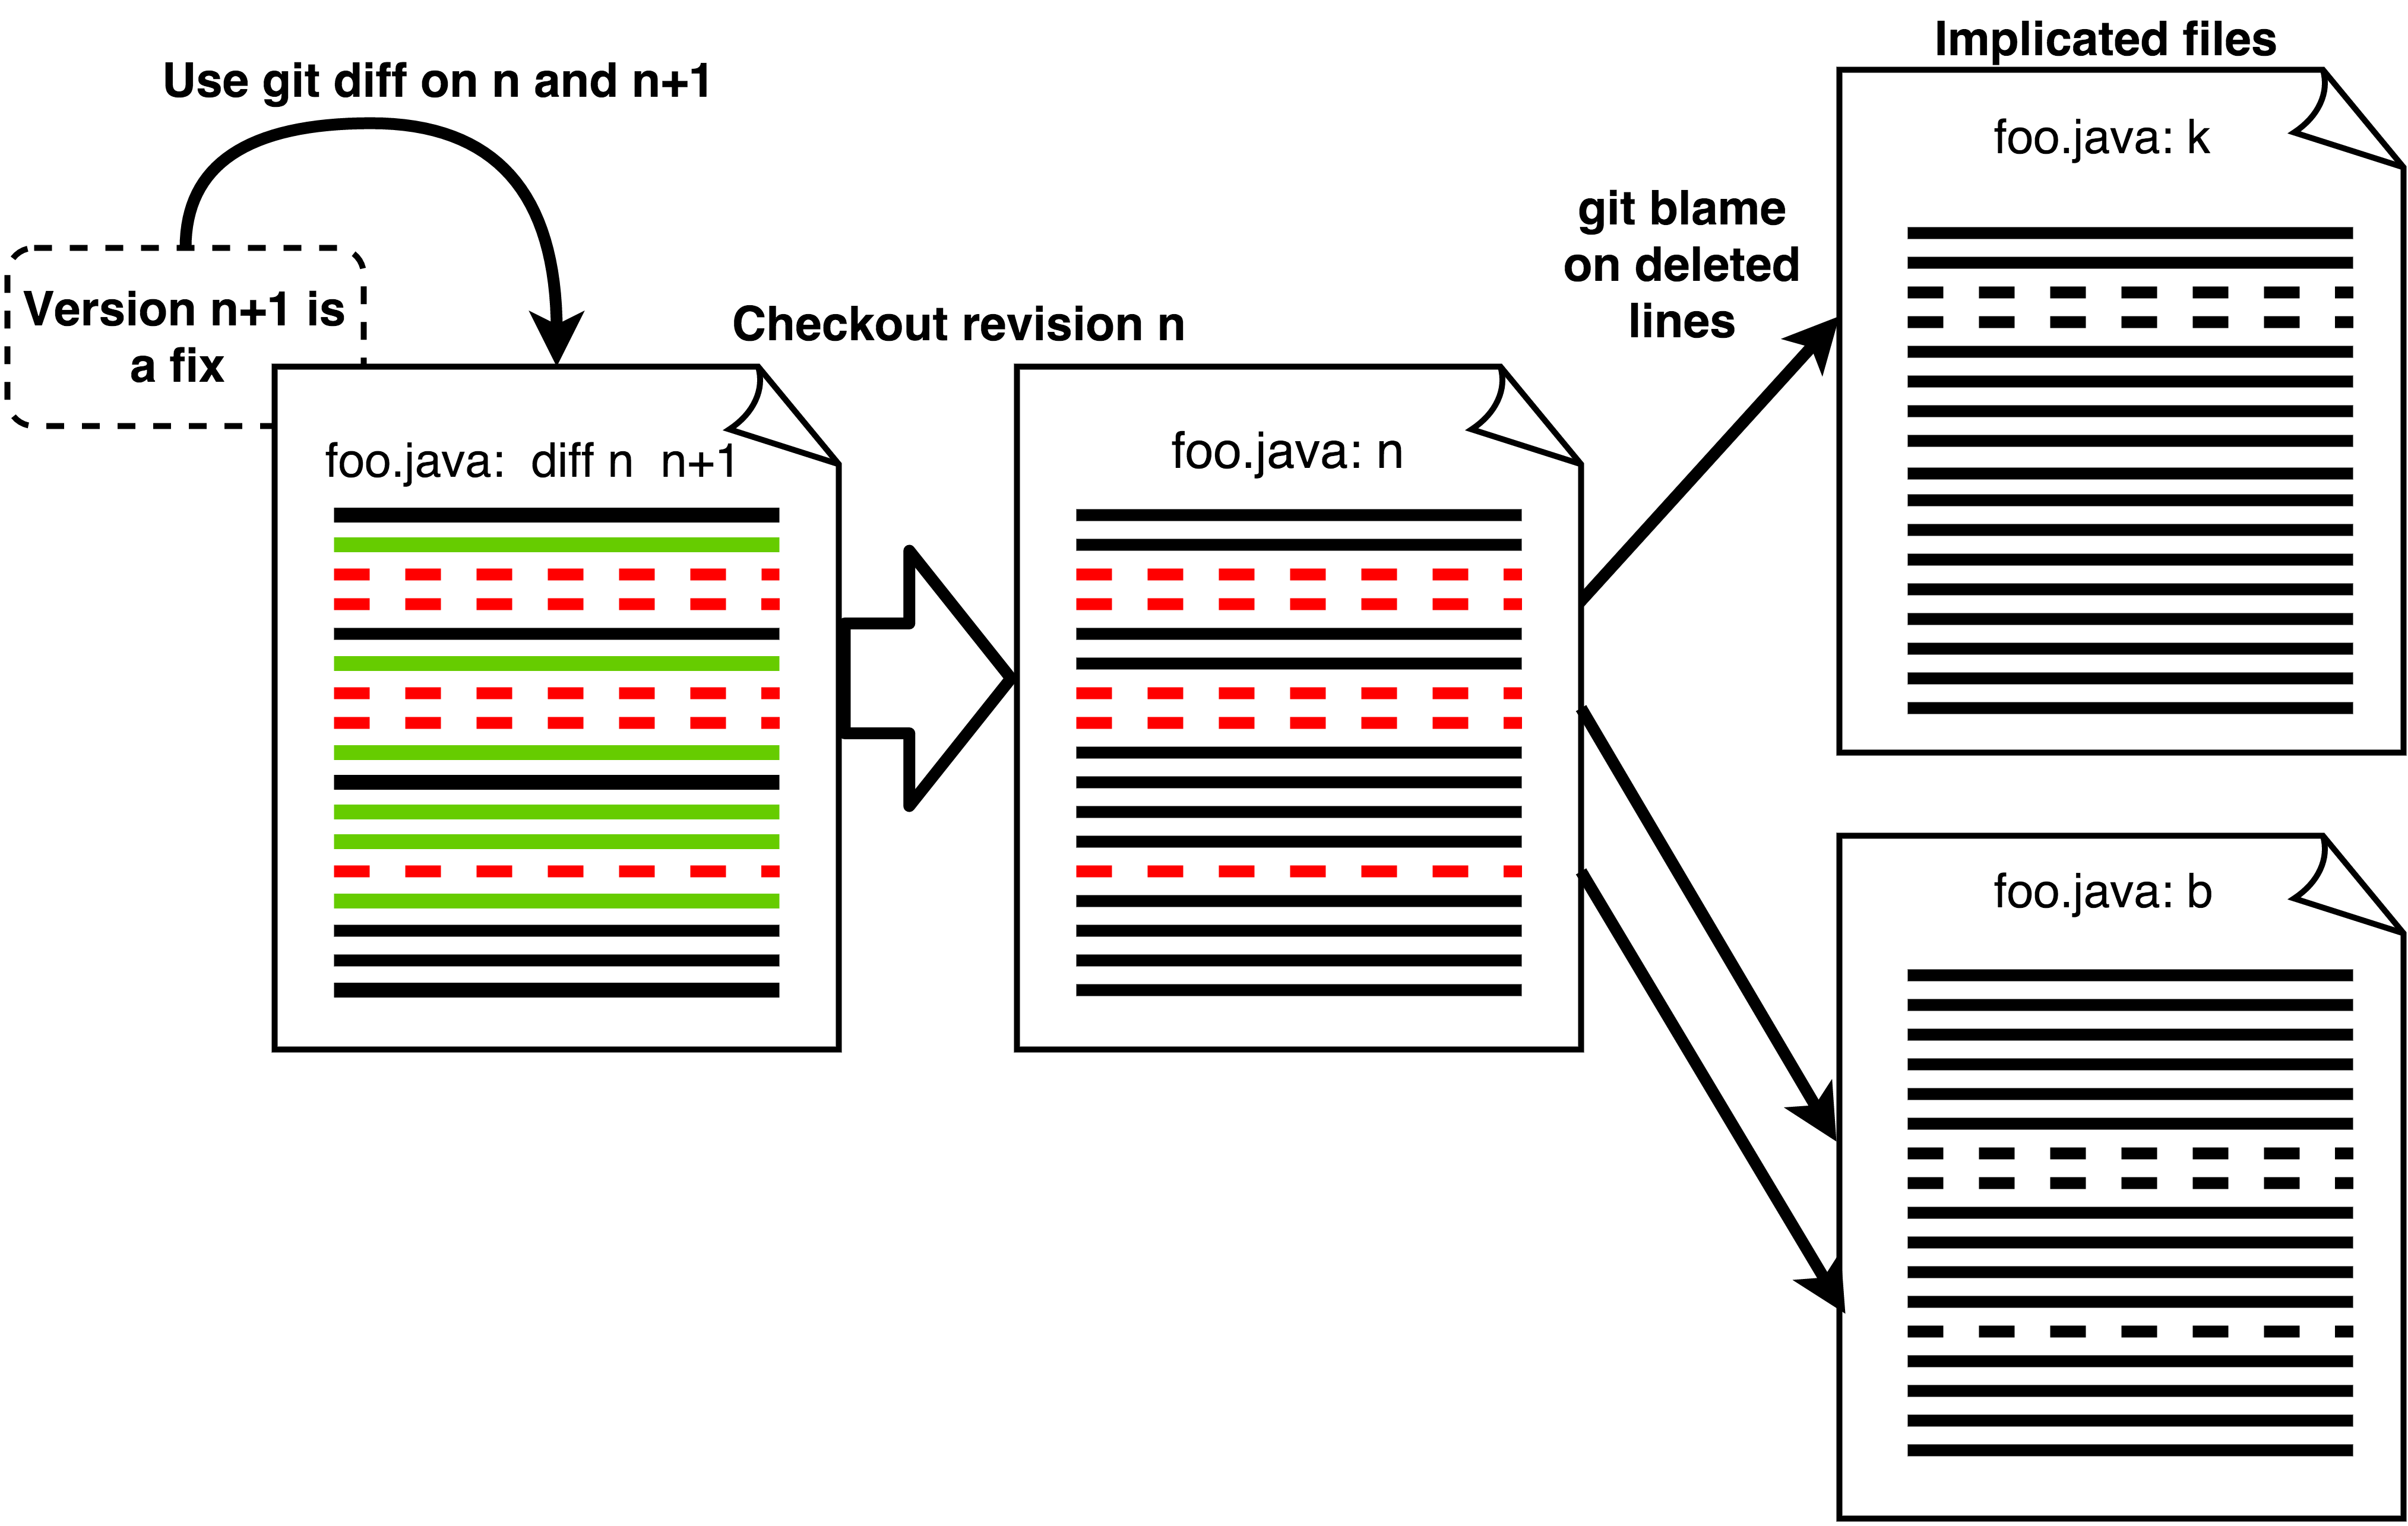
\includegraphics[width=\columnwidth]{images/implicated.png}
    \caption{Implicated code identification technique}
    \label{fig:implicated}
\end{figure}

In this work we don't consider the last step: this because we assume that if the lines are added after the issue reporting date, they are still based on a defective file, and so they contribute to the defect. We want to highlight the fact that a line of code is marked as implicated only in the version of the file in which it is introduced.

Since we need to spot defective file versions we define the new concept of \textbf{implicated file}: a file in a specific version is implicated if that version contains implicated code.

\subsection{Bug and commit linking technique}
\label{sec:bug-linking}
To apply the technique described to extract the implicated files we must be able to identify which commits are bug fixes. To do so we decided to use the JIRA issue tracking system~\footnote{\url{atlassian.com/software/jira}} and in particular the bug convention that Apache projects use on it~\footnote{\url{issues.apache.org/jira/secure/BrowseProjects.jspa\#all}}. Every Apache software project that uses JIRA has an issue key that is, by convention, mentioned in commits that address an issue, together with the issue id. In particular, the convention is to include these information with the following notation: KEY-ID (e.g. LUCENE-1234 if the commit addresses the issue 1234 of the Lucene project).

We consider a commit as a bug fix if its message mentions the key and id of an issue that is marked as a fixed bug on JIRA. To navigate through the JIRA issues we use the data extracted in JSON format in the work by

<MISSING: Cite the technical report for the JIRA JSON issues extraction.>


\subsection{Ownership metrics}
\label{sec:ownership-metrics}
As ownership metrics we decided to compute the ones defined by Bird et al.~\cite{bird:original} and already described in Section~\ref{sec:existing_solutions}. In particular we compute the first three ones (Ownership, Minor and Major) using three different variables to quantify code changes: commit count, number of lines added and number of lines deleted. We also use five different thresholds to distinguish minor and major contributors: 5\%, 10\%, 20\%, 30\% and 40\%. In this way we address also the second and the third of the problems described Section~\ref{sec:existing_solutions}.

To expand our study we also decided to compute the \textit{authorship}. Authorship can be seen as memory-less ownership: the metrics of this class are not based on the history of the development but only on the content of the file on which they are computed. The concept of authorship was already introduced by Rahman et al.~\cite{Rahman:blame}, but was applied only to implicated code chunks and not at a file level. In particular we  compute the two following metrics:
\begin{itemize}
    \item Line authorship: proportion of lines in the file authored by the developer with the highest proportion of lines authored;
    \item Total authors: total number of authors of the lines in the file.
\end{itemize}

We consider these two measures as part of our ownership metrics, following the memory-less vision described above.
To clarify the difference between the two classes of metrics lets suppose to compute them on the version V of the file F, using the number of lines added as variable to quantify the code changes:
\begin{itemize}
\item the proportion of ownership of the contributor C is computed as the number of lines added to F by C over all the considered history (all the versions of F that precede V), divided by the total number of lines added to F by all the contributors over all the considered history;
\item the proportion of authorship of the contributor C is computed as the number of lines that are actually in F in its version V and that are authored by C, divided by the size of F in the same version (in terms of lines);
\end{itemize}

\subsection{Classification}
\label{sec:classification-overview}
As already stated previously in this section, we use the concept of implicated code to mark code that can be considered defective, therefore in this research the defective files are the implicated ones. This means that the classification model that we want to build should distinguish which versions of the project files are implicated using the metrics that we described. 

To be able to evaluate our results in a way that is more sound in the defect prediction field, we first build a model that uses some classic code metrics that are known to be effective, then we add our metrics and we quantify the improvement in the model accuracy (a similar approach was also adopted by Bird et al.~\cite{bird:original}).

The classic metrics that we decided to use are (1) file size; (2) comment-to-code ratio; (3) number of previous defects (implications, in our case). We selected these three because are known to be indicative of software defects~\cite{Rahman:2013, d2012evaluating}.